% Native dvisvgm paths for latex; preserve the PDF driver for pdflatex.
\ifdefined\pdfoutput
  \ifnum\pdfoutput=0 \def\pgfsysdriver{pgfsys-dvisvgm.def}\fi
\fi
\documentclass[tikz,border=8pt]{standalone}
\usepackage{amsmath,amssymb}
\usetikzlibrary{arrows.meta}
\definecolor{positive}{HTML}{C66A20}
\definecolor{negative}{HTML}{2773B4}
\begin{document}
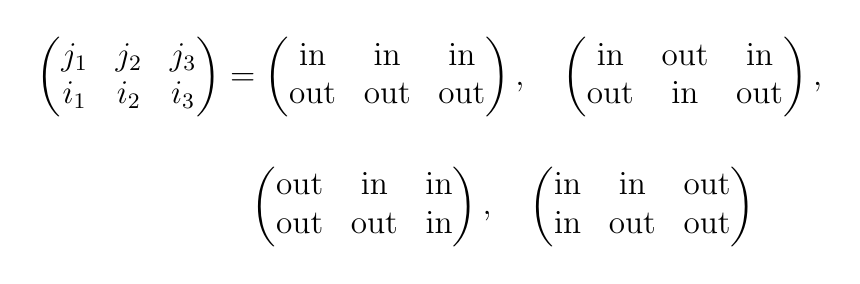
\begin{tikzpicture}[font=\large,line width=.9pt,>={Stealth[length=5pt,width=5pt]},line cap=round,line join=round]
\node {$\displaystyle
\begin{aligned}
\begin{pmatrix}j_1&j_2&j_3\\ i_1&i_2&i_3\end{pmatrix}
&=\begin{pmatrix}\mathrm{in}&\mathrm{in}&\mathrm{in}\\\mathrm{out}&\mathrm{out}&\mathrm{out}\end{pmatrix},\quad
\begin{pmatrix}\mathrm{in}&\mathrm{out}&\mathrm{in}\\\mathrm{out}&\mathrm{in}&\mathrm{out}\end{pmatrix},\\[1.2em]
&\phantom{=}\begin{pmatrix}\mathrm{out}&\mathrm{in}&\mathrm{in}\\\mathrm{out}&\mathrm{out}&\mathrm{in}\end{pmatrix},\quad
\begin{pmatrix}\mathrm{in}&\mathrm{in}&\mathrm{out}\\\mathrm{in}&\mathrm{out}&\mathrm{out}\end{pmatrix}
\end{aligned}$};
\end{tikzpicture}
\end{document}
